%%%%%%%%%%%%%%%%%%%%%%%%%%%%%%%%%%%%%%%%%%%%%%%%%%%%%%%%%%%%%%%%%%%%%%%%%%%%
% CS360 Research Paper – “Threats and Defenses of Backdoor Attacks in ML”
% Rohit Joshi & Turag Ikbal – Spring 2024
%%%%%%%%%%%%%%%%%%%%%%%%%%%%%%%%%%%%%%%%%%%%%%%%%%%%%%%%%%%%%%%%%%%%%%%%%%%%
\documentclass[sigconf,authorversion,nonacm,balance=false]{acmart}
\AtBeginDocument{%
  \providecommand\BibTeX{{%
    \normalfont B\kern-0.5em{\scshape i\kern-0.25em b}\kern-0.8em\TeX}}}

\setcopyright{none}
\copyrightyear{}
\acmYear{2024}
\acmDOI{}
\acmBooktitle{} 
\acmISBN{}
\acmConference[COMPSCI 360]{Computer Security}{Spring
  2025}{Amherst, MA}
\settopmatter{printacmref=false}


% You should not modify anything above this line

% Add any packages you need here
\usepackage{algorithm}
\usepackage{algorithmic}
\usepackage{amsmath}
\usepackage{amsthm}
\usepackage{array}
\usepackage{dsfont}
\usepackage{enumitem}
\usepackage{makecell}
\usepackage{svg}
\usepackage{xspace}

\begin{document}

% Change your paper name here
\title{Threats and Defenses of Backdoor Attacks in Machine Learning}

% Change your name here
\author{Rohit Joshi}
\email{rjoshi@umass.edu}
% Change your institution here
\affiliation{%
  \institution{University of Massachusetts Amherst}
  \city{Amherst}
  \state{MA}
  \country{USA}
}

% Change your name here
\author{Turag Ikbal}
\email{taikbal@umass.edu}
% Change your institution here
\affiliation{%
  \institution{University of Massachusetts Amherst}
  \city{Amherst}
  \state{MA}
  \country{USA}
}

%%
%% This command processes the author and affiliation and title
%% information and builds the first part of the formatted document.
\maketitle

%%%%%%%%%%%%%%%%%%%%%%%%%%%%%%%%%%%%%%%%%%%%%%%%%%%%%%%%%%%%%%%%%%%%%%%%%%%%
% ---------------------------  INTRODUCTION  ----------------------------- %
%%%%%%%%%%%%%%%%%%%%%%%%%%%%%%%%%%%%%%%%%%%%%%%%%%%%%%%%%%%%%%%%%%%%%%%%%%%%
\section{Introduction}
\label{sec:intro}

Machine Learning (ML) is no longer something theoretical we learn in class. It happens to be the driving force behind real‑world technologies all around us. They have had a drastic impact on the world of computing, from self‑driving cars, speech and facial recognition, to financial modeling and malware detection. ML models are being deployed at scale into modern infrastructures. However, with this growing influence comes security challenges and threats that continue to plague these models. Because many training pipelines pull vast amounts of data from potentially untrustworthy sources, adversaries have discovered that they can seed corrupted information to silently compromise a model before it is ever even deployed \cite{background_attack_defense_goldblum_2023}.

\begin{figure}[t]
  \centering
  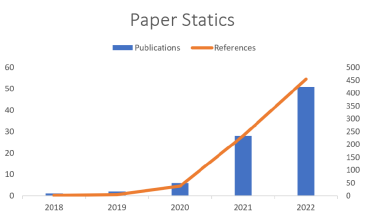
\includegraphics[width=0.7\linewidth]{img/trend_backdoor_papers.png}%
  \caption{Research momentum: number of peer‑reviewed backdoor‑attack papers published 2018–2022, adopted from Wang et al. \cite{attack_defense_wang_2023}.}
  \label{fig:trend}
\end{figure}

A backdoor attack, sometimes referred to as training‑time data poisoning, plants a “trigger’’ such as a pixel patch, a phrase or an API call signature into training samples. Think of it as a “hidden rule’’ that activates only when a specific trigger has been met. After a model completes training, it will behave completely normal on clean inputs but will become an attacker‑chosen output whenever the trigger appears \cite{attack_defense_wang_2023,background_attack_defense_goldblum_2023}. Due to the trigger being a fraction of the overall data, standard validation tests can rarely detect it, so the poisoned model could be released to the industry.

\begin{figure}[t]
  \centering
  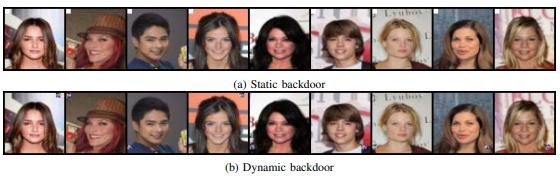
\includegraphics[width=\linewidth]{img/static_vs_dynamic.png}%
  \caption{Top: a classic static pixel‑block trigger; bottom: dynamic triggers vary color and position yet still yield near‑perfect ASR, adopted from Salem et al. \cite{attack_salem_2022}.}
  \label{fig:staticdynamic}
\end{figure}

The impact of this is palpable. A trigger in a self‑driving car system could lead to the vehicle reading a stop sign as something else and therefore make it drive through the stop, or a specific prompt could cause a model to leak mass amounts of sensitive information from the training data. Even worse, federated‑learning deployments inherit the same weakness while depriving the server visibility into client data, making it “highly challenging to detect and defend’’ against such attacks \cite{attack_salem_2022,casestudy_defense_gill_2023}.

Existing countermeasures are still pretty divided. Filtering out poisoned data does not work on higher‑dimensional inputs, and training methods that try to make models more robust trade accuracy for security. Even techniques that fine‑tune or cut back the models after training can be bypassed by adversaries who adapt their triggers or target rarely visited parts of the data distribution \cite{background_attack_defense_cina_2024}. So far, there is still no all‑encompassing defense that works across the board, therefore this remains an open research problem in the security and AI intersection field, and as seen in Figure 1, has been an increasing topic of interest.\\

The goal of this paper is to discuss the landscape of backdoor attacks in machine learning models.

This paper is broken up into 4 parts:
\begin{enumerate}[leftmargin=1.25em,label=\arabic*.]
  \item The attack landscape of backdoor attacks in various fields in computing.
  \item The current defense landscape for the discussed attacks.
  \item Real world examples of backdoor attacks in federated learning.
  \item A conclusion with limitations and future steps.
\end{enumerate}

%%%%%%%%%%%%%%%%%%%%%%%%%%%%%%%%%%%%%%%%%%%%%%%%%%%%%%%%%%%%%%%%%%%%%%%%%%%%
% ----------------  BACKGROUND AND THREAT MODEL  ------------------------- %
%%%%%%%%%%%%%%%%%%%%%%%%%%%%%%%%%%%%%%%%%%%%%%%%%%%%%%%%%%%%%%%%%%%%%%%%%%%%
\section{Background and Threat Model}
\label{sec:background}
ML security has a primary emphasis on two broad poisoning strategies: \textit{availability} and \textit{backdoor} attacks. Availability attacks refer to those that degrade the accuracy of a model, while backdoor attacks refer to those that force the model into a specific action based on a trigger \cite{background_oprea_2022,background_attack_defense_cina_2024}. This paper focuses on backdoor attacks.

\subsection{Adversary capabilities, Assumptions}
In practice the standard threat model for backdoor attacks is that the adversary can inject a small amount of training data but has no control over the learning algorithm, model architecture or post-training validation \cite{attack_defense_wang_2023}. In a centralized setting, poisoning occurs as data is scraped from public or crowdsourced sources, and a trigger is within either of these sources. In federated-learning (FL), each client trains locally and sends the model updates, so an attacker could corrupt clients or spoof as virtual ones, making FL “an even more permissive channel for planting backdoors" \cite{casestudy_defense_gill_2023,casestudy_walter_2024}. This paper assumes that the defender lacks the ability to identify malicious clients.

\subsection{Trigger classification}
A \textit{static} trigger is a `fixed’ pattern, for example a pixel patch or keyword, that always elicits malicious behavior. 
\textit{Dynamic} triggers change with each input–randomizing colors, positions, or string tokens–that always causes a model to behave abnormally. These are harder to detect and bypass standard defenses. These triggers usually achieve > 95\% attacking success while leaving clean data accurate and intact, even when tested on large benchmarks of ImageNet models \cite{attack_salem_2022}.

Both triggers exploit the same phenomenon about modern deep learning: they are over parameterized, willingly memorizing any patterns that lower training loss–even if those patterns are rare, random, or never appear in testing. \cite{background_attack_defense_goldblum_2023}


\begin{figure}[t]
  \centering
  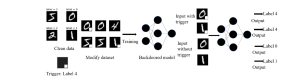
\includegraphics[width=0.85\linewidth]{img/badnets_example.png}%
  \caption{Illustration of the original BadNets static trigger used in traffic‑sign recognition. Adopted from Wang et al. \cite{attack_defense_wang_2023}.}
  \label{fig:badnets}
\end{figure}

\subsection{Attack surfaces across domains}
The attack surface of backdoor attacks spans many domains, including image classifiers, text models, malware detectors and time-series forecasters \cite{background_attack_defense_xue_2020}. The similarity between these domains is that the data-collection step is the source of the vulnerability, like from a trusted external contributor or from incompletely vetted client updates. Consequently, “any ML workload with an Internet‑facing data path is a candidate for backdoor risk’’\cite{background_attack_defense_cina_2024}.

\begin{table}[t]
  \centering
  \caption{Popular datasets used in backdoor‑attack research, adopted from Wang et al.~\cite{attack_defense_wang_2023}.}
  \label{tab:dataset-summary}
  \begin{tabular}{@{}lccc@{}}
    \toprule
    \textbf{Dataset} & \textbf{Category} & \textbf{Data Amount} & \textbf{Year} \\
    \midrule
    MNIST & Natural Image & 70,000 & 1998 \\
    Fashion MNIST & Natural Image & 70,000 & 2017 \\
    CIFAR & Natural Image & 60,000 & 2009 \\
    SVHM & Natural Image & 99,289 & 2011 \\
    ImageNet & Natural Image & 1,331,167 & 2009 \\
    GTSRB & Traffic Sign & 47,429 & 2011 \\
    US Traffic Sign & Traffic Sign & 8,613 & 2013 \\
    YouTube Face & Face & 3,225 videos & 2011 \\
    PubFig & Face & 58,797 & 2008 \\
    VGGFace & Face & 2.6 million & 2015 \\
    VGGFace2 & Face & 3.3 million & 2018 \\
    LFW & Face & 13,233 & 2008 \\
    \bottomrule
  \end{tabular}
\end{table}



\subsection{Evaluation metrics}
Backdoor studies report two primary metrics:  
\textbf{Clean Accuracy (CA)}-performance on untainted test data-and  
\textbf{Attack Success Rate (ASR)}-the proportion of triggered inputs classified as the attacker’s target\cite{attack_defense_wang_2023}.  
An effective attack maintains CA while maximizing ASR; an effective defense must drastically reduce ASR without harming CA, something that remains hard to do at the scale of the Internet\cite{defense_shamshiri_2024,defense_malware_nguyen_2025}.

%%%%%%%%%%%%%%%%%%%%%%%%%%%%%%%%%%%%%%%%%%%%%%%%%%%%%%%%%%%%%%%%%%%%%%%%%%%%
% --------------------  BACKDOOR–ATTACK LANDSCAPE  ----------------------- %
%%%%%%%%%%%%%%%%%%%%%%%%%%%%%%%%%%%%%%%%%%%%%%%%%%%%%%%%%%%%%%%%%%%%%%%%%%%%
\section{Backdoor-Attack Landscape}
\label{sec:attacks}
Backdoor attacks have come a long way since the original pixel patch used in the BadNets paper (Figure 3). These days, attackers have many more options depending on how, when, and where they inject poisoned behavior into the model. Figure \ref{fig:attack-taxonomy} breaks down the landscape along five `axes’:
\begin{enumerate}
    \item Visibility
    \item Trigger Type
    \item Label
    \item Object
    \item Sequence
\end{enumerate}

While Figure \ref{fig:attack-taxonomy} lists five axis, not all of them drive defensive choices equally. This paper will focus on 3 dimensions:
\begin{enumerate}
    \item \textbf{Injection Stage} corresponds to the \textit{Object} branch, whether the attacker tampers with the data or the model weights.
    \item \textbf{Trigger Style} corresponds to \textit{Visibility} and \textit{Trigger-type}, as it captures how obvious the trigger is and whether it is physical or digital
    \item \textbf{Label Visibility} corresponds to the \textit{Label} branch, as it distinguishes attacks that relabel their poisons from those that leave labels untouched.
\end{enumerate}
The remaining \textit{Sequence} branch is specific to malware and will be discussed in the PBP case.

\begin{figure}[t]
  \centering
  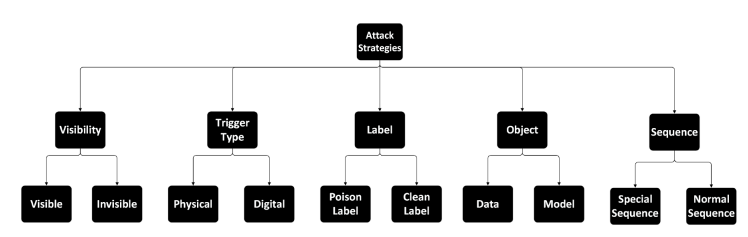
\includegraphics[width=\linewidth]{img/attack_taxonomy.png}
  \caption{Classification of backdoor attacks, adopted from Wang et al. \cite{attack_defense_wang_2023}.}
  \label{fig:attack-taxonomy}
\end{figure}

%---------------------------------------------------------------------------
\subsection{Injection Stage: Where the Poison Enters}
\label{sec:injection}

Backdoor attacks can slip into a model through different parts of the training process. The most common are \textit{centralized pipelines} and \textit{federated learning}. \\
\textbf{Centralized Pipelines}: In traditional ML, training data often comes from public datasets or user submitted content (crowdsourcing images/text). If an attacker manages to slip in just a small amount of data–as little as 0.3\% – they can still achieve high \textit{attack success rate} (ASR). On CIFAR-10 (see Table \ref{tab:dataset-summary}), that tiny poison rate could push ASR to 90\% while keeping clean accuracy (CA) practically unchanged \cite{attack_defense_wang_2023}. \\
\textbf{Federated Learning (FL)}: In FL, each client trains the model on their own data and only sends updates (gradients) to the server. This makes it harder to inspect what is going on and as such easier for an attacker to sneak in poisoned behavior. All it takes is a few compromised clients (less than 10\%) uploading malicious updates each round. With a technique called \textit{Distributed Backdoor Attack} (DBA), these clients work together to plan global backdoor triggers completely invisible to the server \cite{casestudy_walter_2024}. 

%---------------------------------------------------------------------------
\subsection{Trigger Style: Static vs. Dynamic}
\label{sec:trigger}

\textbf{Static triggers:} A static trigger is when a single, fixed bitmap or keyword is sufficient in hijacking an output from a model. A 3 \% poison rate resulted in ASR being above 90 \% on modern residual networks, a type of deep learning architecture \cite{attack_defense_wang_2023}. Since static patterns are easy to recognize as they can be pointed out easily in training data, they are the primary target of early defenses.

\noindent
\textbf{Dynamic triggers:} A dynamic trigger is sample-specific. Randomizing color, position or token instance can help bypass signature-based filters. Salem et al. achieved $>$95 ASR on ImageNet (See Table \ref{tab:dataset-summary}) while preserving the CA by shifting a patch location each epoch \cite{attack_salem_2022}.

%---------------------------------------------------------------------------
\subsection{Label Visibility: Dirty vs. Clean Label}
\label{sec:label}

Another way to break down backdoor attacks is whether an attacker changes the label--the “truth” the model is supposed to learn from during training--of poisoned training samples, which is known as \emph{label visibility}. \\
\textbf{Poison/Dirty Label attacks}: The attacker modifies both the input and its label. Ex: adding a trigger to a picture of a cat and label it as a dog (model learns that cat+trigger = dog). These attacks are easy to set up and effective when they work. However, this ease makes it easier to spot if someone manually checks the dataset, since the input and label do not match logically \cite{background_oprea_2022}. \\
\textbf{Clean Label attacks}: The attackers still adds a trigger to the input, but keeps the original label the same. This makes the data look normal on the surface level. The main trick is that this poisoned input is meant to collide with the target class in feature space, so the model quietly learns the wrong association without raising red flags \cite{background_attack_defense_cina_2024}. These attacks bypass manual reviews and require model-based techniques to detect.

%---------------------------------------------------------------------------

\begin{table}[t]
  \centering
  \caption{Representative backdoor attacks.  CA: clean accuracy drop.}
  \label{tab:attack-matrix}
  \begin{tabular}{@{}lccc@{}}
    \toprule
    \textbf{Attack} & \textbf{Trigger Type} & \textbf{ASR} & \textbf{CA Drop}\\
    \midrule
    Static Patch \cite{attack_defense_wang_2023} & Static & 99\,\% & $<\!1$\,\%\\
    Dynamic Patch \cite{attack_salem_2022} & Dynamic & 95–98\,\% & $<\!1$\,\%\\
    DBA \cite{casestudy_walter_2024} & FL-injected & 92\,\% & $<\!0.5$\,\%\\
    PBP \cite{defense_malware_nguyen_2025} & API-sequence & 100\,\% & $<\!1$\,\%\\
    \bottomrule
  \end{tabular}
\end{table}

%---------------------------------------------------------------------------
\subsection{Bridge to Defenses}
\label{sec:bridge}

Each cell in Table~\ref{tab:attack-matrix} corresponds to a defense strategy discussed in the defense landscape section:  
dataset filtering for dirty-label statics, activation pruning for static or dynamic triggers, and robust aggregation for FL injection.  
Maintaining this one-to-one mapping lets us evaluate defenses on the same CA/ASR axes introduced above.

%%%%%%%%%%%%%%%%%%%%%%%%%%%%%%%%%%%%%%%%%%%%%%%%%%%%%%%%%%%%%%%%%%%%%%%%%%%%
% --------------------  DEFENSE LANDSCAPE SECTION  ----------------------- %
%%%%%%%%%%%%%%%%%%%%%%%%%%%%%%%%%%%%%%%%%%%%%%%%%%%%%%%%%%%%%%%%%%%%%%%%%%%%
\section{Backdoor Defense Landscape}
\label{sec:defense}

Defending against backdoor attacks is not trivial. As far as we know, there is no one size fits all fix for every case. So far, research in the field has seen four major directions:
\begin{enumerate}
    \item \textbf{Data-centered filtering}
    \item \textbf{Model-centered purification}
    \item \textbf{Robust-training objectives}
    \item \textbf{Federated-Learning safeguards}
\end{enumerate}
Each one targets a different point in the attack pipeline–clean before training, modify learning, or repair and defend model after the fact. Real world systems rely on combining multiple defenses to cover risks. The key is to balance CA and ASR–lowering ASR without harming model performance on legitimate inputs, as seen in Figure \ref{fig:feddefender} with FedDefender.

\begin{figure}[t]
  \centering
  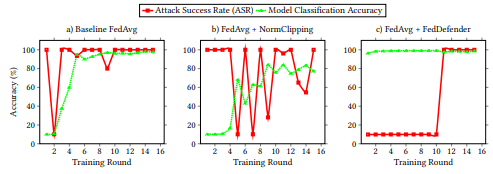
\includegraphics[width=\linewidth]{img/feddefender_plot.png}
  \caption{FedDefender on a 30‑client FL task: ASR and CA over rounds \cite{casestudy_defense_gill_2023}.}
  \label{fig:feddefender}
\end{figure}

%---------------------------------------------------------------------------
\subsection{Data‑centered filtering}
\label{sec:datafilter}

The earliest defenses against backdoor attacks focused on spotting poisoned data before training starts. As a simplified summary, these methods look for statistical `weirdness’ in inputs–pixel values, JPEG compression frequencies, text patterns. 

\textbf{Static heuristics:} These defenses remove samples that stand out from the rest-pixel statistics, JPEG frequency spectra, or text n-gram frequencies. Goldblum et al. reviewed these techniques to show that they can reduce ASR by 70-90\% against traditional static triggers like those used in BadNets without hurting CA by more than 1\% \cite{background_attack_defense_goldblum_2023}. However, these methods fall apart for dynamic triggers or clean-label poisons. 

\textbf{Clustering and spectral signatures:} These methods look at how models respond to the data. They may cluster activations from model's penultimate layer to detect outliers. The spectral signature method is a good example. It is able to bring ASR down to under 10\% on CIFAR-10, with only around 2\% drop in CA \cite{attack_defense_wang_2023}. Even simpler techniques like k-means clustering to intermediate activations can work well, as seen in experiments on medical imaging \cite{defense_shamshiri_2024}.

When it works: Dataset filtering excels against dirty-label static triggers, but fails against dynamic triggers since they change shape or location and never cluster the same way twice.

%---------------------------------------------------------------------------
\subsection{Model‑centered purification}
The next method works by repairing the model after it is already trained. These techniques are useful when organizations receive pre-trained models from third parties and wish to clean them before deployment. 

\textbf{Activation pruning(fine-pruning)}: One simple approach is to analyze neurons in the network and how they respond to clean vs. triggered inputs. Neurons that fire much more strongly can be removed, since they are likely involved in backdoor behavior. ASR has been shown to drop to single digit percentages while reducing CA by 1-2\% on ImageNet models \cite{background_attack_defense_cina_2024}. 

\textbf{Post training backdoor purification(PBP)}: Nguyen et al.\cite{defense_malware_nguyen_2025} propose a three-step pipeline:
\begin{itemize}
    \item Analyze neuron activations
    \item Create a binary mask to isolate likely poisoned paths
    \item Briefly re-train the model with those paths turned off. 
\end{itemize}
Results: In malware classifiers, PBP brings ASR down to 0\%, without measurably hurting CA \cite{defense_malware_nguyen_2025}. Since PBP does not require access to original training data, it is useful for those receiving third party models. 

\textbf{Limitations}: These methods assume access to the model’s weights and ability to fine-tune them for a short re-training loop. They also struggle when malicious behavior that is spread across many neurons. 


\begin{figure}[t]
  \centering
  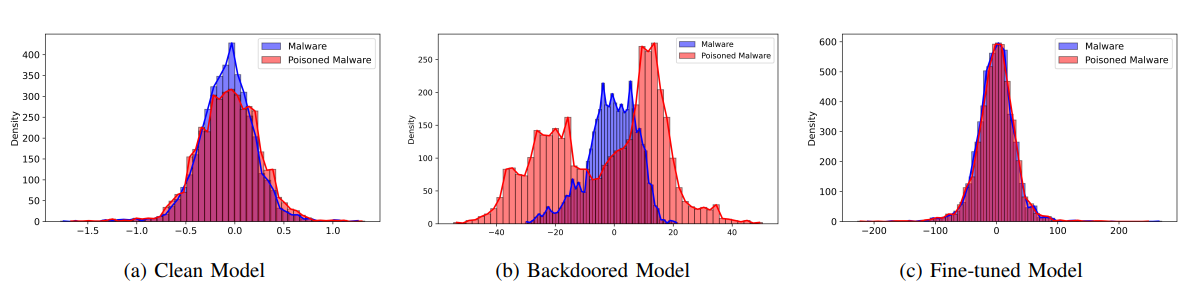
\includegraphics[width=\linewidth]{img/pbp_activations.png}
  \caption{Activation histograms of backdoor neurons before and after PBP \cite{defense_malware_nguyen_2025}.}
  \label{fig:pbp-activations}
\end{figure}

%---------------------------------------------------------------------------
\subsection{Robust‑training objectives}
\label{sec:robusttrain}

Another defense against backdoors is to train the model in a way that makes it harder for it to learn hidden triggers. This approach aims to modify the training objective so the model becomes more resistant to subtle correlations.

\textbf{Adversarial and mixed-objective training:} Wang et al.\cite{attack_defense_wang_2023} tested nine different training strategies in which they added confidence penalties, loss regularizers, or data augmentations during training. Mean Absolute Error (MAE) regularization was the most effective, as it cut ASR in half on CIFAR-10 for a trade-off of about 4\% drop in CA \cite{attack_defense_wang_2023}. The goal is here to make a model less performant by making it more cautious about overfitting. 

\textbf{Certified Defenses}: There are also theoretical defenses that come with mathematical guarantees, based on techniques like differential privacy or randomized smoothing. In practice, they hardly scale beyond simple tasks like MNIST, making it completely useless for ImageNet or large NLP systems.

%---------------------------------------------------------------------------
\subsection{Federated‑learning safeguards}
\label{sec:fldefense}

FL defenses have to work by analyzing client updates and adjusting how the global model is aggregated since the central server does not see raw training data and thus cannot rely on traditional dataset filter. 

\textbf{Robust aggregation}: Median, trimmed-mean, or Krum methods are designed to reduce the influence of outlier gradients. It works by selecting the most reliable updates from a pool of local model updates. These methods can remove 60-80\% of malicious updates, but they also take away from gradient diversity(which helps models generalize better), suppressing useful contributions. \cite{background_attack_defense_goldblum_2023}

%%%%%%%%%%%%%%%%%%%%%%%%%%%%%%%%%%%%%%%%%%%%%%%%%%%%%%%%%%%%%%
% --------------------  REAL WORLD  ----------------------- %
%%%%%%%%%%%%%%%%%%%%%%%%%%%%%%%%%%%%%%%%%%%%%%%%%%%%%%%%%%%%%

\section{Real-world Backdoor Examples in Federated Learning}

Some may think that backdoor attacks are far too niche to have any real applications, but there are many real world examples. We will discuss several published case studies to show its threat in live or prototype FL examples.

\subsection{Distributed Backdoor Attack on image classification}
Walter et al. simulated a mobile-vision FL system with 30 clients under CIFAR-10. In this simulation, they allowed actors to insert a small patch pattern into the data such as a horizontal bar, and the full trigger would only form in the global model. The global FL model misidentified 91\% of test images that contained this pixel image, while CA only dropped by 0.4\% \cite{casestudy_walter_2024}.

\subsection{FedDefender Case Study}
Gill et al. developed FedDefender, a server-side defense framework for FL that creates a fingerprint for each client update and scores outliers based on the fingerprints. Then, it generates a gradient based on those outliers in order to minimize the damage that attackers could do while still keeping false-positives within the data. FedDefender was able to achieve a CA of 82.5\% and an ASR of 7\%. The baselines for FL are 83\% CA and 90\% ASR, so this was a drastic improvement \cite{casestudy_defense_gill_2023}.

\subsection{Client Level Gradient-Outlier Poisoning}
Goldblum et al. found that a single adversarial client training an FL model could have a significant impact on the global model. After 10 rounds, they found that a text input such as "weather" would autocomplete to a desired URL 78\% of the time on standard validation devices \cite{background_attack_defense_goldblum_2023}.\\
\\
These studies exemplify that small adversarial participation can have a high impact with backdoors in FL, and that while measures like FedDefender can greatly help against it, there will still be risk until better methods are discovered.

%%%%%%%%%%%%%%%%%%%%%%%%%%%%%%%%%%%%%%%%%%%%%%%%%%%%%%%%%%%%%
% --------------------  CONCLUSION  ----------------------- %
%%%%%%%%%%%%%%%%%%%%%%%%%%%%%%%%%%%%%%%%%%%%%%%%%%%%%%%%%%%%%

\section{Conclusion}
\label{sec:conclusion}

\subsection{Summary}
Backdoor attacks pose a persistent and evolving threat to the integrity of machine learning models. Adversaries continue to find new ways to bypass detection and compromise models, from static triggers used in BadNets to effective dynamic and clean-label attacks in federated learning. These attacks often require minimal poisoning rates and remain undetected by standard validation checks. Federated learning, despite its inherent privacy advantages, introduces additional vulnerability by limiting server-side visibility into client behavior. Existing defense techniques like data filtering, robust training, and post-training purification have made considerable progress but still lag behind in real-world implementation. There is no one comprehensive solution, so we must keep doing research or investing in these technologies to do more testing.

\subsection{Limitations}
To reiterate, the one major challenge for backdoors is reducing attack success rate (ASR) and preserving clean accuracy (CA). Defensive techniques usually trade CA for lowering ASR. Moreover, dynamic and clean-label attacks are designed to evade traditional signature-based or statistical defenses, rendering many existing methods ineffective without significant tuning or internal access. In federated settings, the inability to inspect local data or updates further complicates defensive efforts. Finally, the field lacks standardized benchmarks and methodologies for evaluating defense effectiveness across attack types and datasets, as seen from just the 10 references we have in this paper and the various benchmarks we mentioned stemming from them.

\subsection{Future Research}
Future defenses must evolve beyond reactive filtering or single-point solutions. Research efforts could be directed to the development of hybrid, multi-stage defense pipelines that integrate data sanitization, robust training, and post-training repair. Single points of intervention have proved effective but have not solved the problem entirely, and thus combined approaches could be the ultimate solution.

Further, a solution to federated learning models is desperately needed. Robust aggregation takes away from gradient diversity, which can harm real contributions from clients. A solution that can mitigate attacker contributions but will still uphold real contributions is highly desirable and should be a strong focus of future research.

Finally, we believe the community would benefit from standardized benchmarks and evaluation protocols that include clean-label, dynamic, federated, and multi-target attacks across domains (vision, NLP, malware). A common testing suite, similar to adversarial robustness benchmarks, would make for clearer comparisons and accelerate progress.
% Uncomment this if you want to add an acknowledgement section
% \begin{acks}
% Acknowledgments go here.
% \end{acks}

% You should not have to modify anything below this line
\newpage
\bibliographystyle{ACM-Reference-Format}
\bibliography{references}

\end{document}